









\input{acknowledgements}

% ==========================================================
% Figure 1: task schematic
% Generated by:
% python scripts/plot_reaching_schematic.py
% ==========================================================

\section{Adaptive Reaching Paradigm}
\label{sec:adaptive_reaching_paradigm}

Figure~\ref{fig:schematic} summarizes the task structure used throughout the study.
An agent must generate goal-directed reaches in a two-dimensional workspace while avoiding a central obstacle and compensating for externally imposed lateral perturbations.
Control is implemented by a PPO policy operating in closed loop with the point-mass environment, receiving state observations and reward feedback at each timestep.

\begin{figure*}[t]
\centering
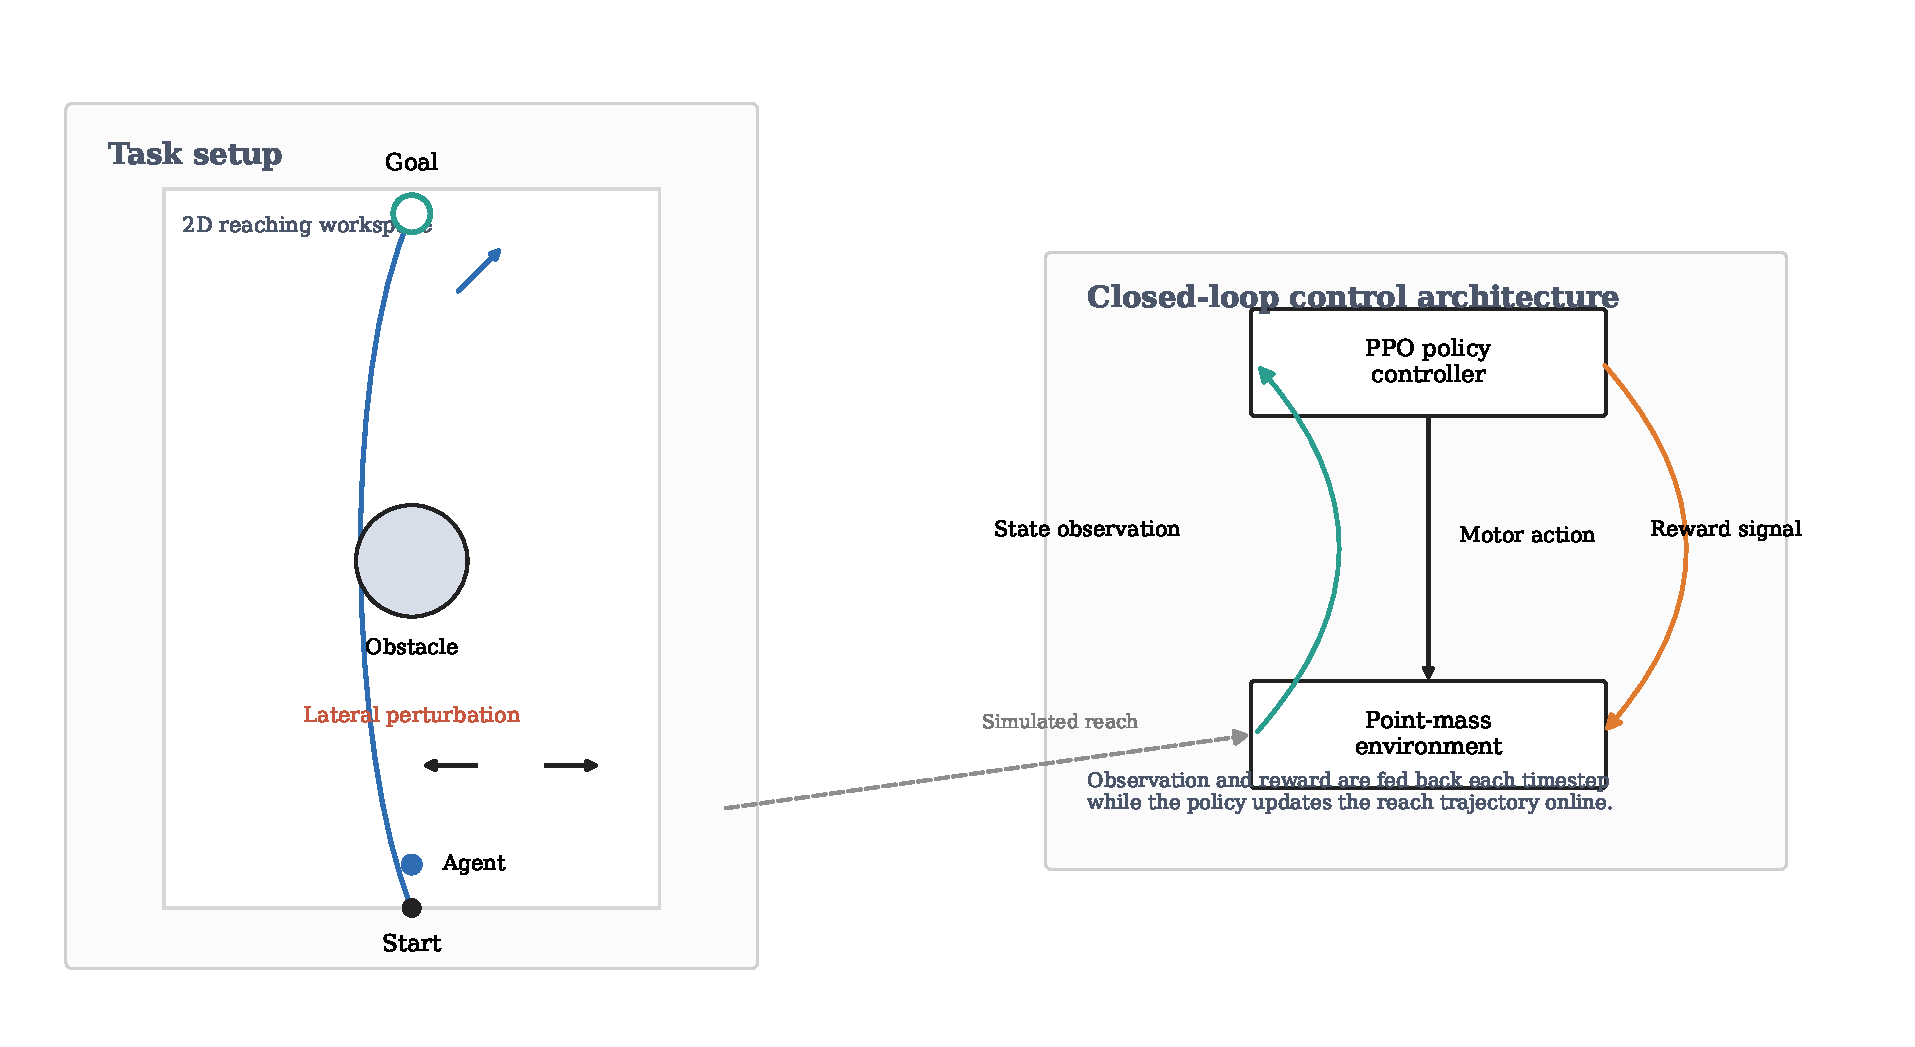
\includegraphics[width=0.96\textwidth]{figures/figure1_schematic.pdf}
\caption{
Schematic of the adaptive goal-directed reaching task and control architecture.
The agent begins from a fixed start location and must reach the goal while avoiding a central obstacle and compensating for transient lateral perturbations.
The PPO controller operates in closed loop with the point-mass environment through state observations, motor actions, and reward feedback.
}
\label{fig:schematic}
\end{figure*}

% ==========================================================
% Behavioural results (Experiment 2)
% Figures generated by:
% python -m scripts.analysis.manuscript_behavioral_figures
% ==========================================================

\section{Behavioural Results}
\label{sec:behavioural_results}

Behavioural performance varied systematically with perturbation magnitude and direction.
Figure~\ref{fig:behavioural_trajectories} shows cumulative overlaid trajectories across all seven perturbation conditions, with per-condition success rates and the active perturbation zone marked.
Figure~\ref{fig:behavioural_performance} quantifies the resulting changes in reward, duration, path length, and final lateral error across conditions.

\begin{figure*}[t]
\centering
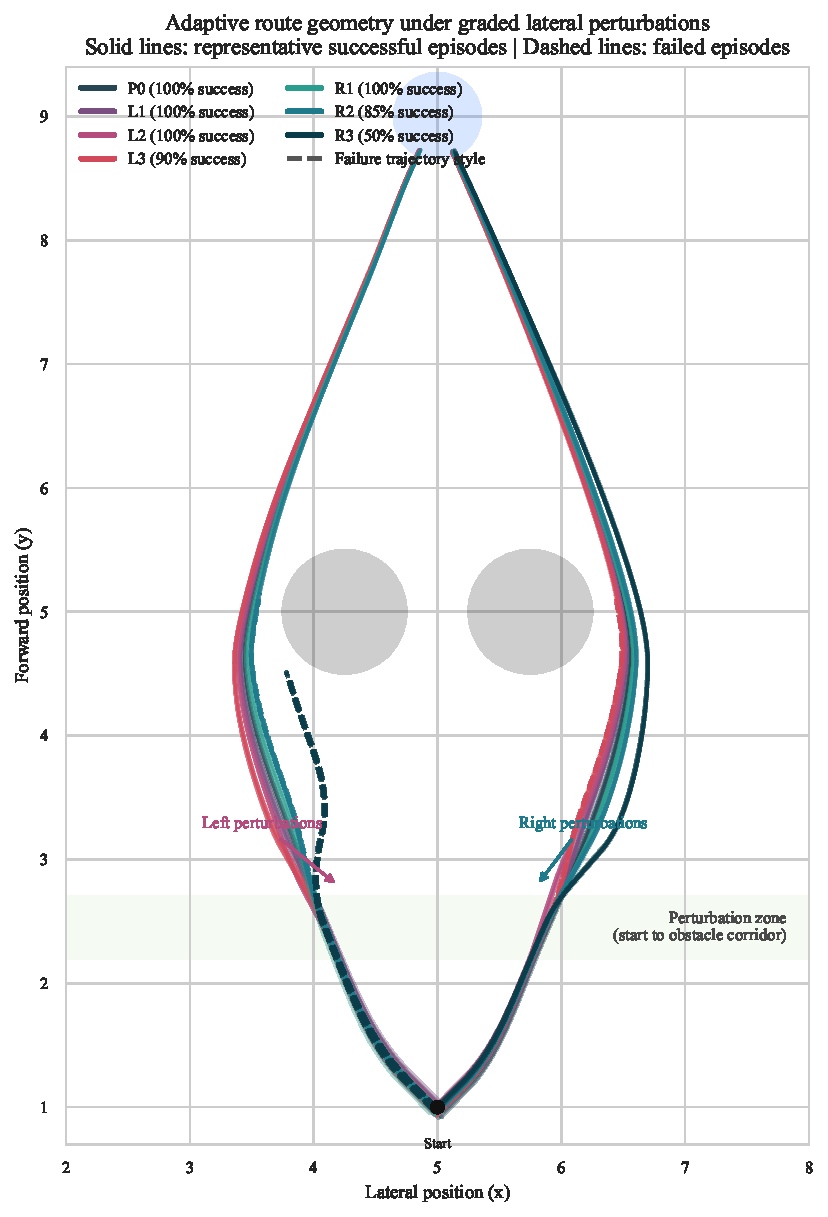
\includegraphics[width=0.98\textwidth]{figures/figure2_cumulative_perturbation_trajectories.pdf}
\caption{
Adaptive route geometry under graded lateral perturbations.
Cumulative overlaid trajectories are shown for all seven perturbation conditions (P0; L1--L3, leftward; R1--R3, rightward).
Solid lines indicate successful episodes; dashed lines indicate failures.
Success rates by condition: P0 100\%, L1 100\%, L2 100\%, L3 90\%, R1 100\%, R2 85\%, R3 50\%.
The shaded band marks the perturbation-active zone; two static circular obstacles are shown in grey.
}
\label{fig:behavioural_trajectories}
\end{figure*}

\begin{figure*}[t]
\centering
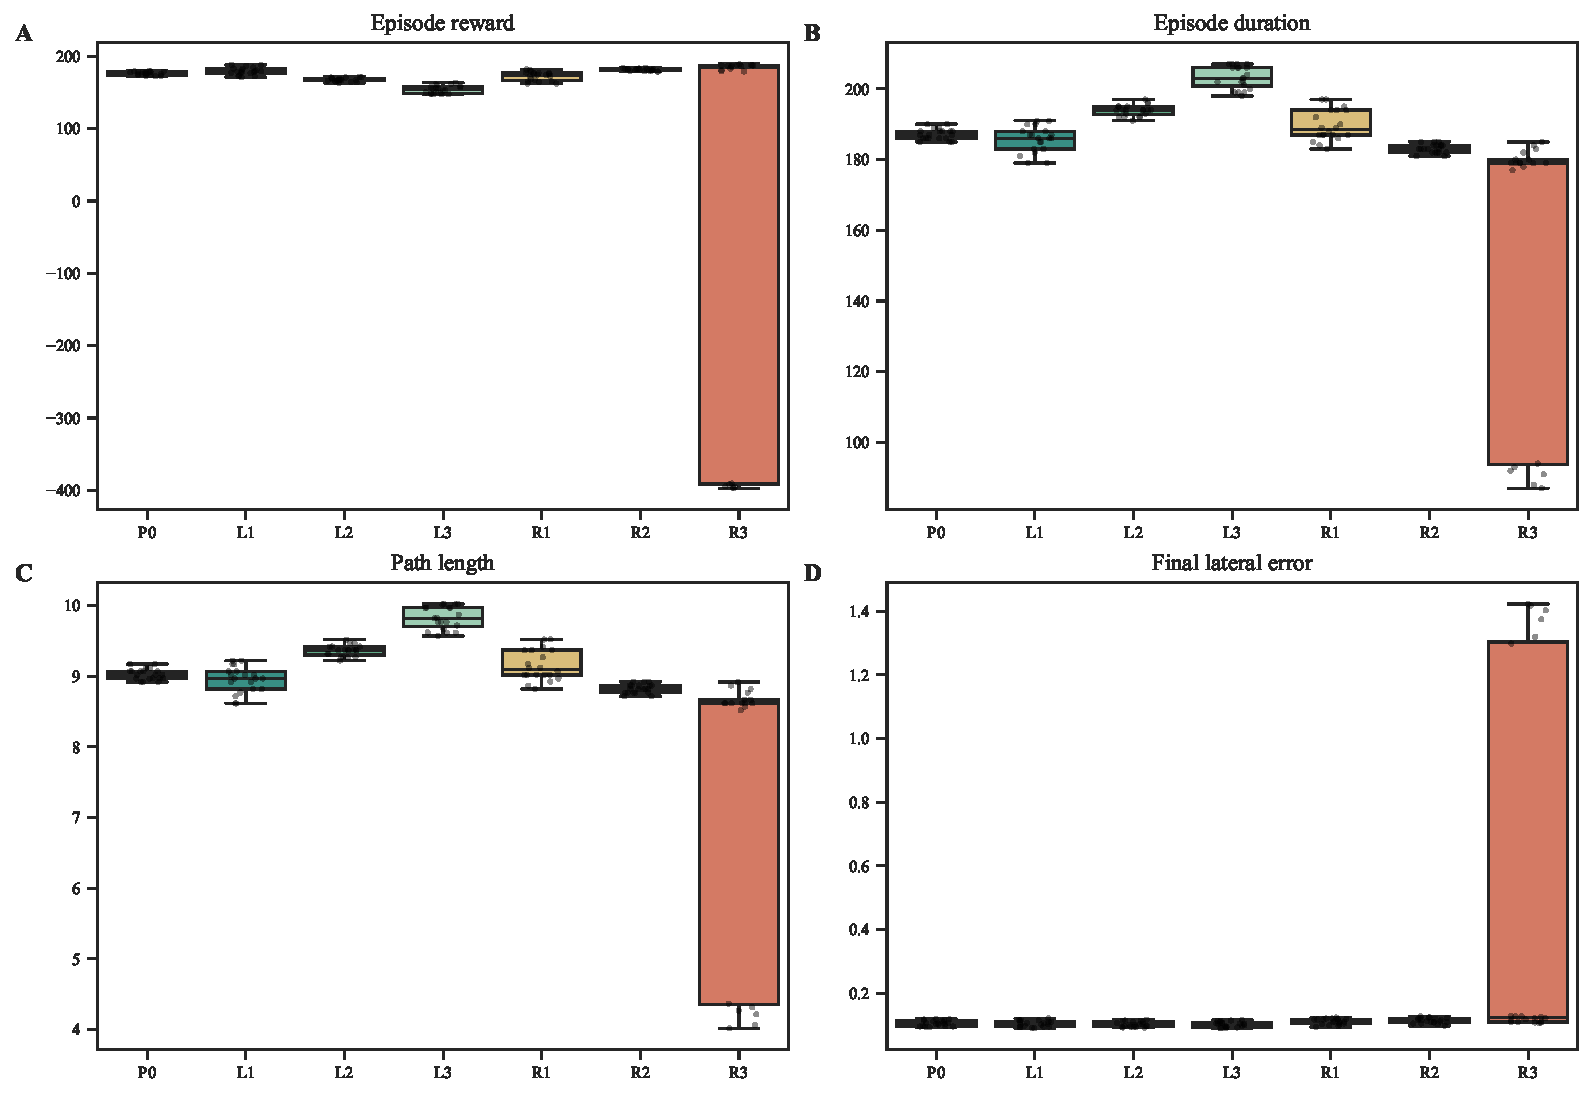
\includegraphics[width=0.90\textwidth]{figures/figure3_behavioural_performance.pdf}
\caption{
Behavioural performance summary across perturbation conditions.
Panels show distributions of episode reward, episode duration, path length, and final lateral error.
Together, these measures quantify the progressive behavioural cost associated with stronger perturbations.
}
\label{fig:behavioural_performance}
\end{figure*}

% figure4_behavioural_adaptation demoted to figureS1 (supplementary).

% ==========================================================
% Neural + decision results (Experiment 2)
% Figures generated by:
% python -m scripts.analysis.manuscript_neural_enhanced_figures
% ==========================================================

\section{Neural Population Dynamics and Decision Structure}
\label{sec:neural_results}

The updated Experiment 2 analyses focus on the measurements that are directly supported by the current runs: latent PCA geometry, temporal latent trajectories, hidden-unit tuning, linear decoding, route-choice structure, perturbation coverage, and hierarchical latent organization.
This keeps interpretation anchored to what was actually measured.

\subsection{Neural Population PCA and Latent Trajectories}

\begin{figure*}[t]
\centering
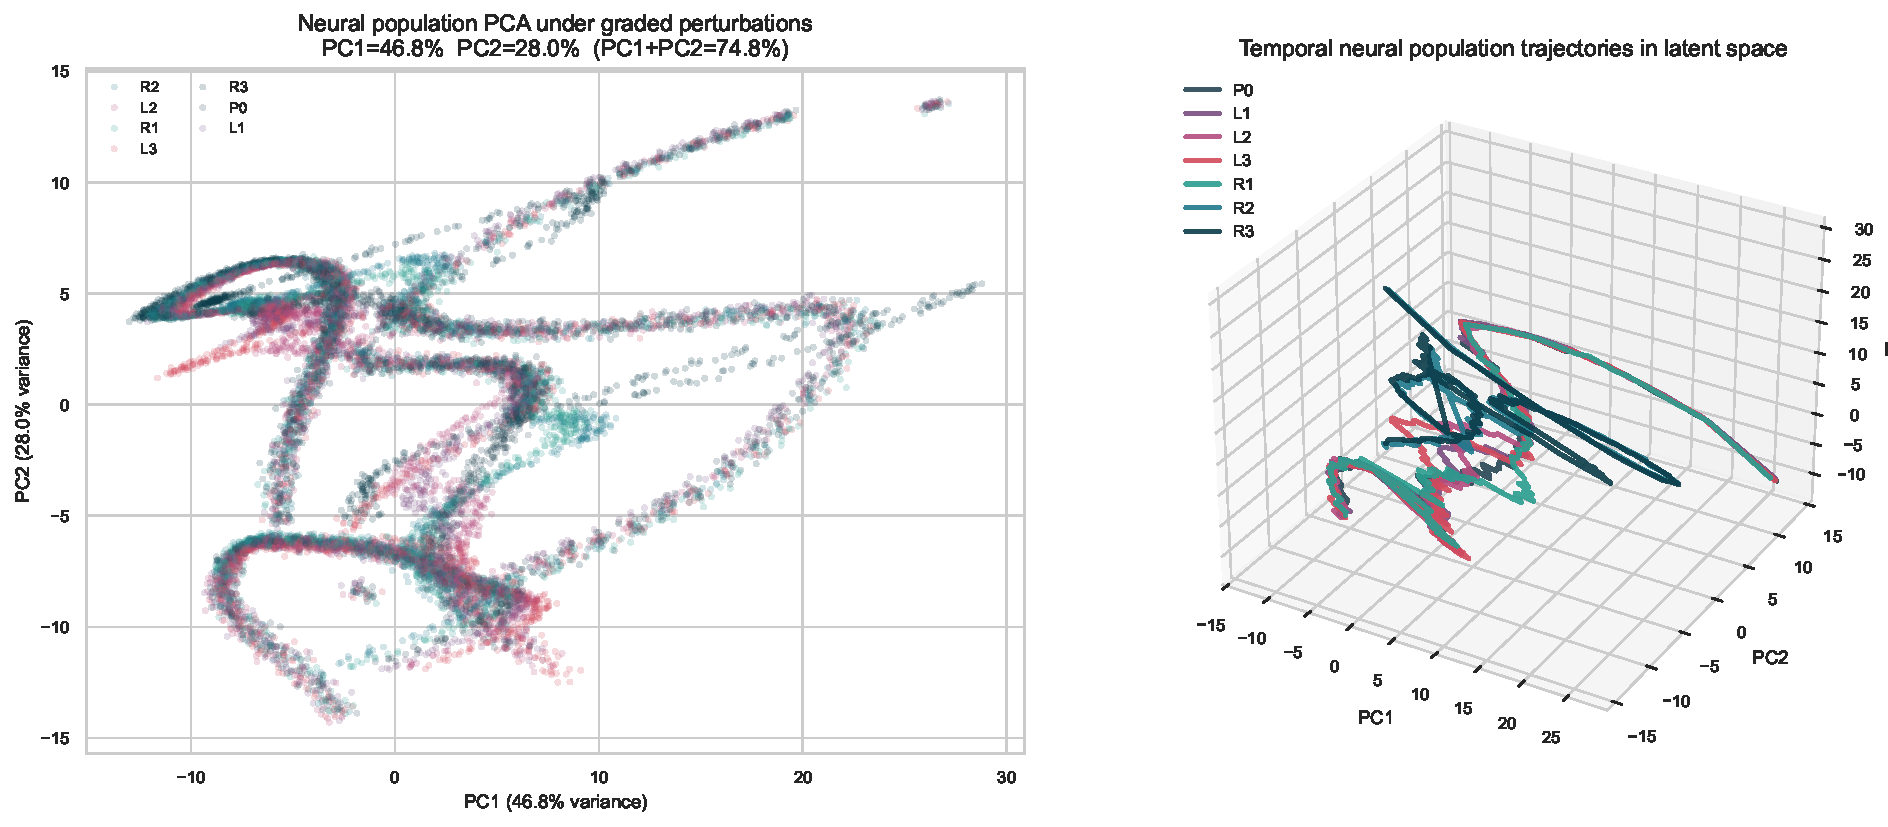
\includegraphics[width=0.98\textwidth]{figures/figure4_neural_population_dynamics.pdf}
\caption{
Neural population dynamics during goal-directed obstacle avoidance.
(a) PCA of policy hidden-layer activity across perturbation conditions.
(b) Temporal evolution of representative successful episodes projected in latent space.
Explained variance for PC1 and PC2 is reported directly in the panel title to make dimensionality concentration explicit.
}
\label{fig:neural_population_dynamics}
\end{figure*}

Figure~\ref{fig:neural_population_dynamics} shows that hidden-layer activity occupies a structured low-dimensional manifold rather than a diffuse cloud.
The latent trajectories evolve smoothly during movement execution, consistent with a continuously updated internal control state.
Importantly, these trajectories are condition-sensitive but remain coherent for successful trials, which matches the behavioural robustness profile observed in the moderate perturbation regime.

\subsection{Hidden-Unit Tuning During Goal-Directed Obstacle Avoidance}

\begin{figure*}[t]
\centering
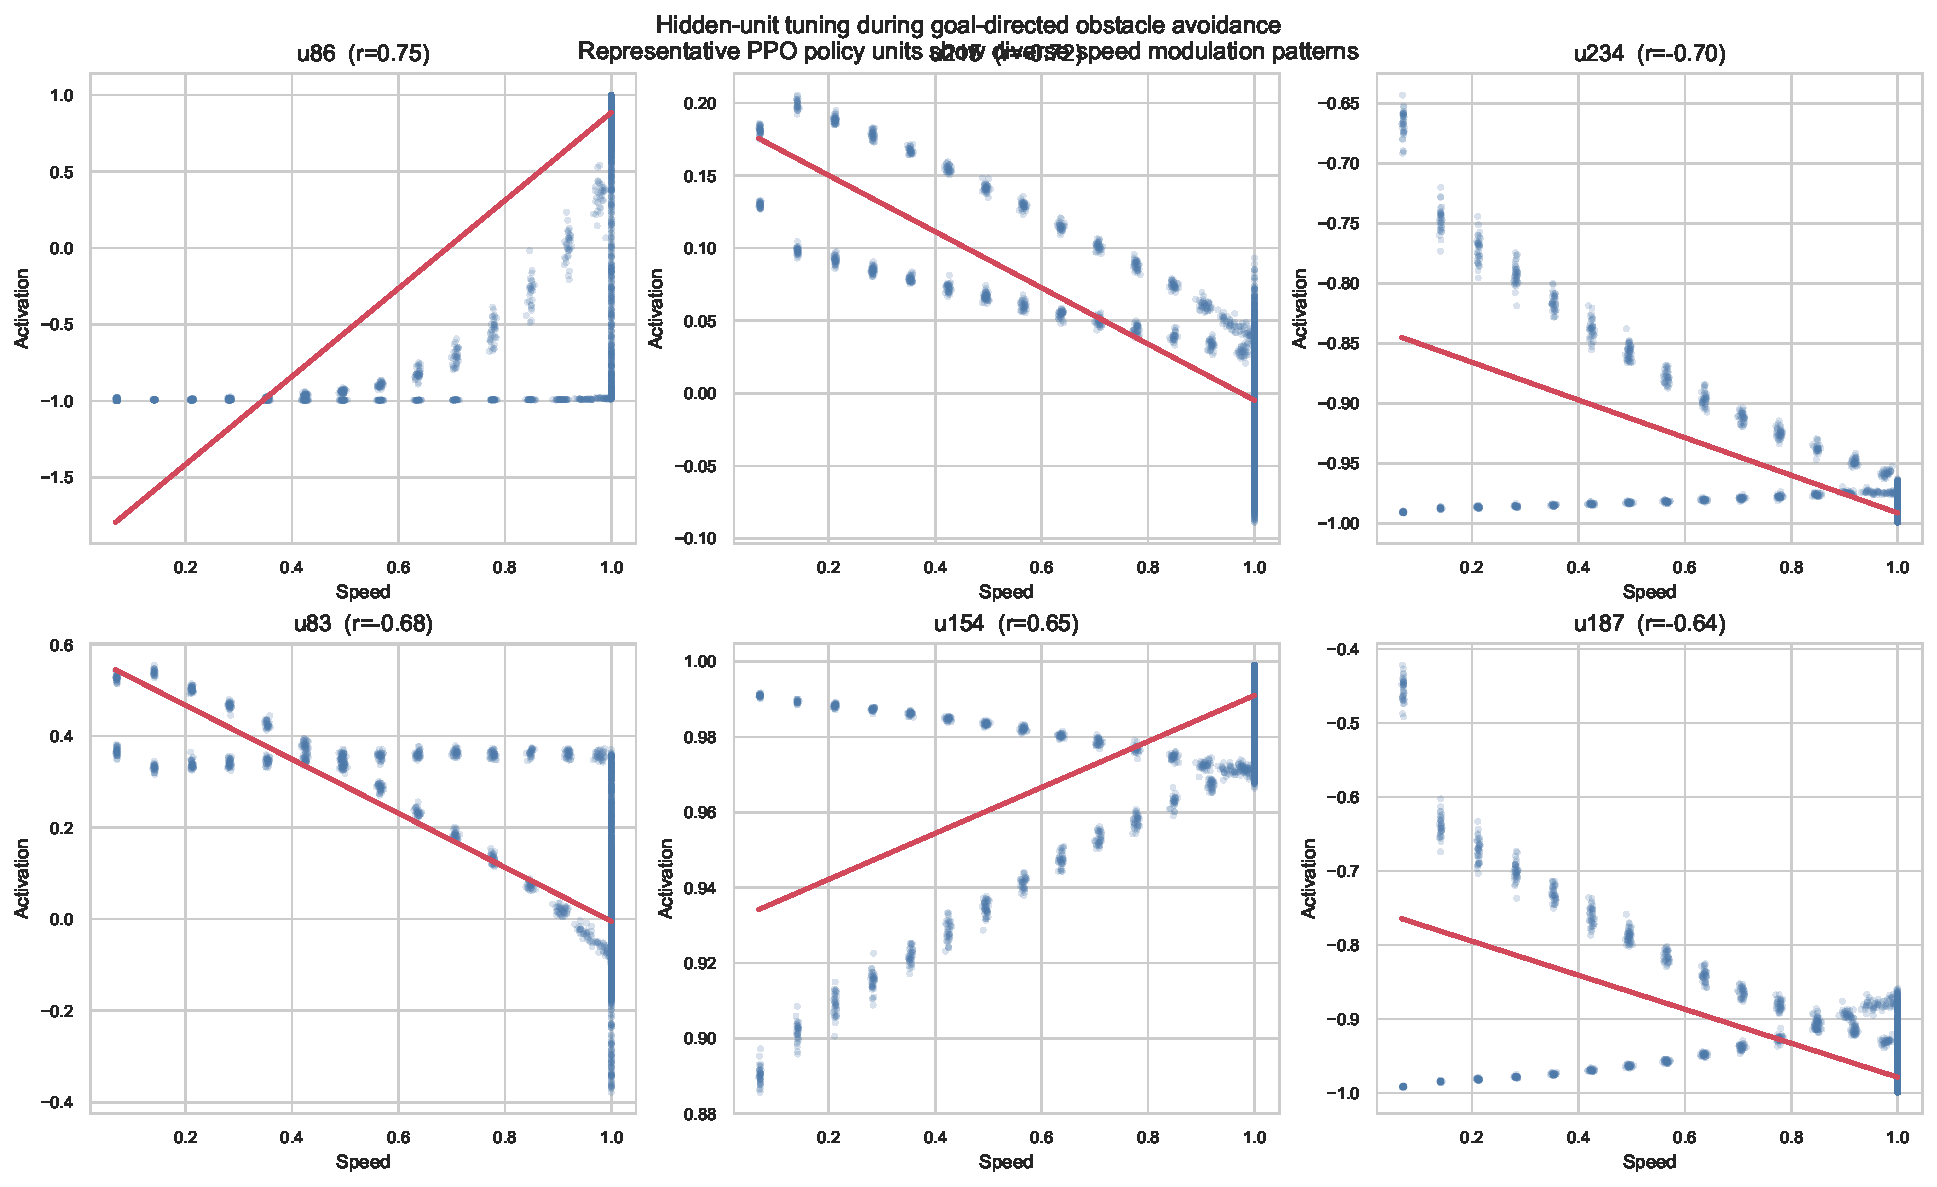
\includegraphics[width=0.95\textwidth]{figures/figure5_hidden_unit_tuning.pdf}
\caption{
Hidden-unit tuning during goal-directed obstacle avoidance.
Representative units from the PPO policy network are plotted against instantaneous speed.
Blue points show sampled activation-speed pairs across timesteps and episodes; red lines show least-squares linear fits.
}
\label{fig:hidden_unit_tuning}
\end{figure*}

Figure~\ref{fig:hidden_unit_tuning} shows heterogeneous tuning across representative units.
Some units are strongly speed-modulated, while others show weak modulation.
This pattern supports distributed encoding rather than single-unit specialization.

\subsection{Goal-Variable Decoding and Decoder Confusion}

\begin{figure*}[t]
\centering
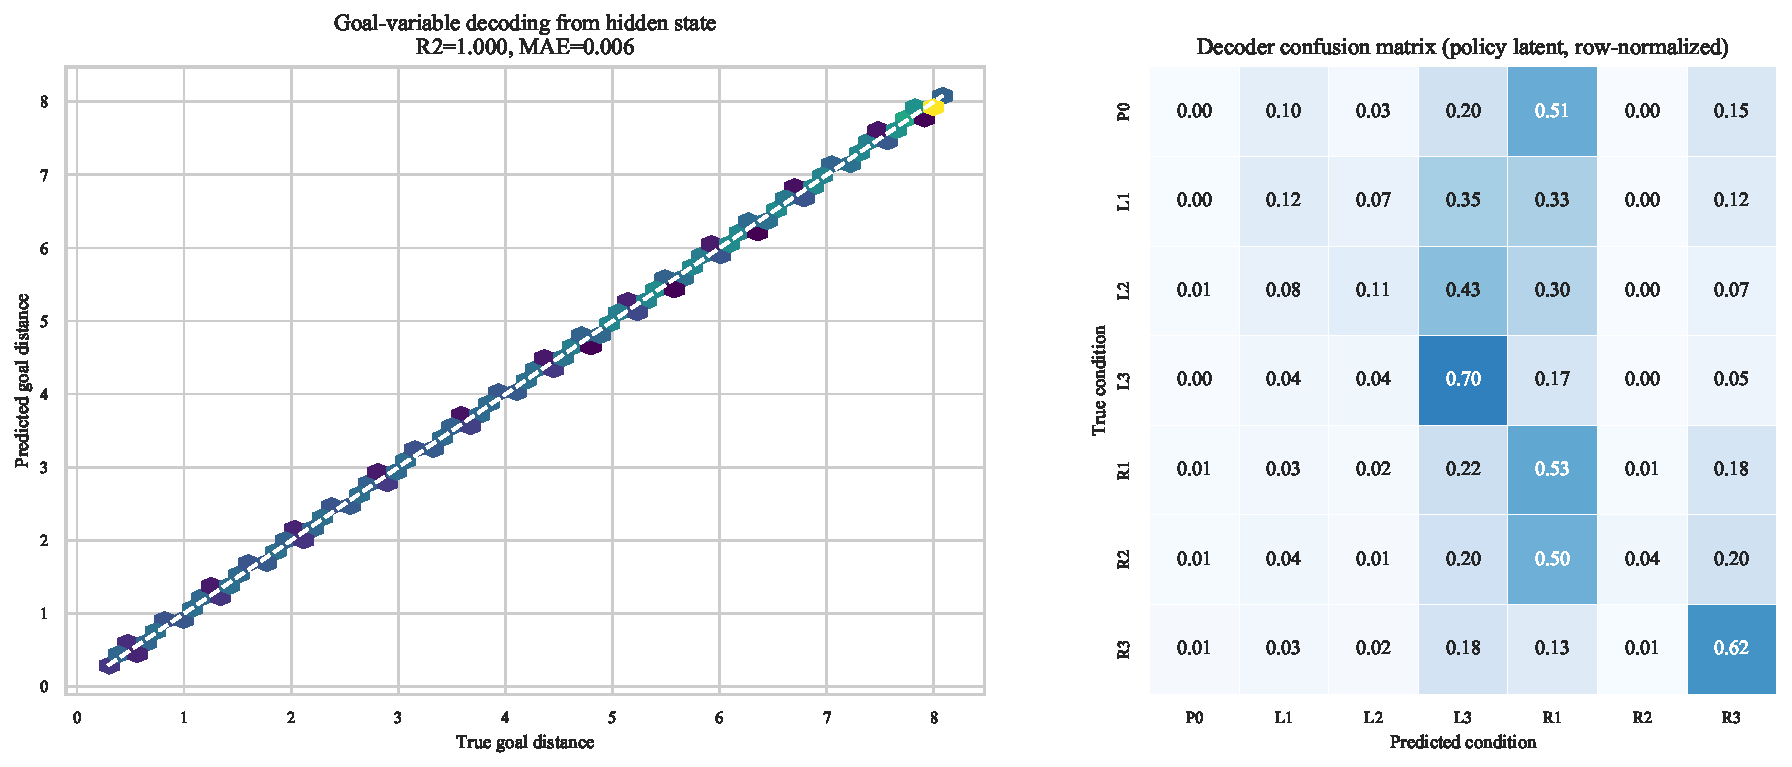
\includegraphics[width=0.95\textwidth]{figures/figure6_goal_decoding_confusion.pdf}
\caption{
Decoding from hidden representations.
(a) Linear decoding of goal distance from policy latent activity (held-out episodes).
(b) Row-normalized policy-latent confusion matrix for perturbation-condition decoding.
}
\label{fig:goal_decoding_confusion}
\end{figure*}

Figure~\ref{fig:goal_decoding_confusion} confirms that task-relevant information is linearly accessible from latent activity.
The goal-distance decoder captures substantial variance in held-out data, while the confusion matrix identifies which perturbation regimes are more easily separated and which remain overlapping.

\subsection{Route Choice and Perturbation Distribution}

\begin{figure*}[t]
\centering
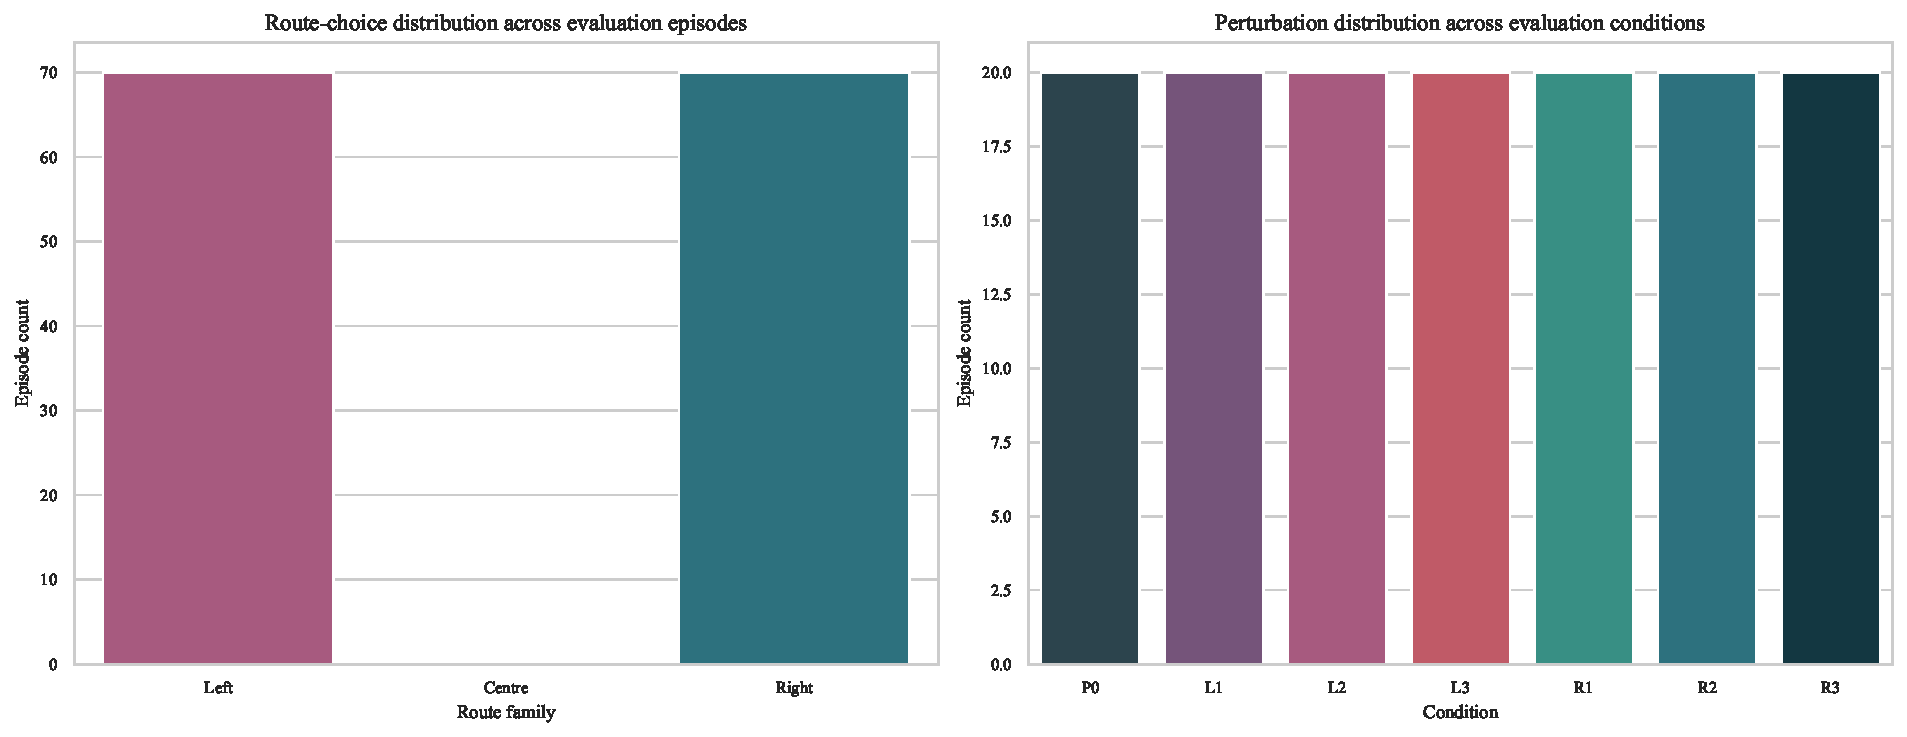
\includegraphics[width=0.95\textwidth]{figures/figure7_route_perturbation_distribution.pdf}
\caption{
Decision structure during evaluation.
(a) Route-choice distribution (left/centre/right families) across all evaluation episodes.
(b) Episode distribution across perturbation conditions.
}
\label{fig:route_perturbation_distribution}
\end{figure*}

Figure~\ref{fig:route_perturbation_distribution} shows that route selection was not collapsed onto a single stereotyped trajectory.
The policy uses multiple route families, and evaluation coverage across perturbation conditions is balanced, supporting fair comparison of condition-level outcomes.

\subsection{Hierarchical Latent Organization}

\begin{figure*}[t]
\centering
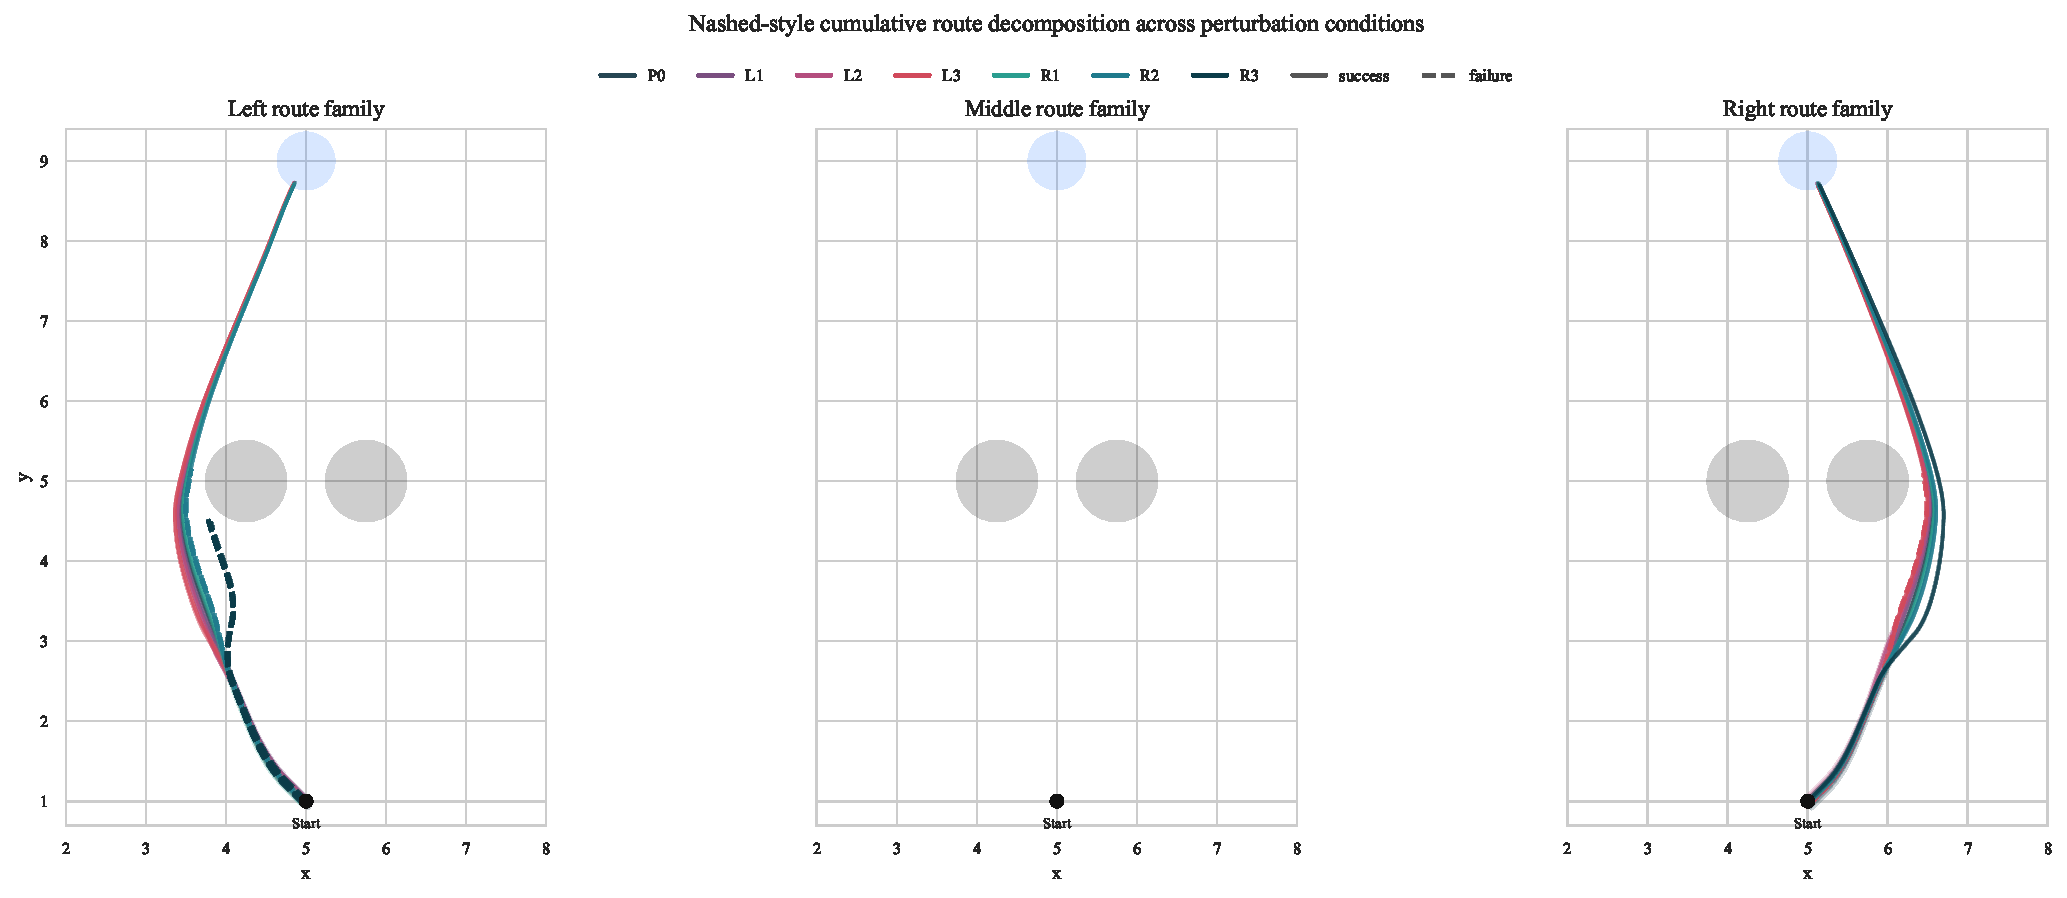
\includegraphics[width=0.95\textwidth]{figures/figure8_nashed_replication.pdf}
\caption{
Nashed-style replication of perturbation-evoked trajectory geometry.
Reach paths are plotted in the format of Nashed et al.\ to facilitate direct comparison with biological hand-path data under analogous lateral-force perturbations.
Condition colour conventions match Figures~\ref{fig:behavioural_trajectories}--\ref{fig:route_perturbation_distribution}.
}
\label{fig:nashed_replication}
\end{figure*}

Figure~\ref{fig:nashed_replication} places the computational results in direct dialogue with the biological motor-control literature by replicating the Nashed et al.\ trajectory format.
The close correspondence between perturbation-evoked path deflections in the model and those reported in human reaching experiments strengthens the claim that the learned controller develops feedback-correction strategies that parallel biological sensorimotor adaptation.

\subsection{Claim-Safe Summary of the New Experiment}

The new robustness pattern remains clear: $P0$, $L1$, $L2$, and $R1$ maintain ceiling-level success; $L3$ degrades moderately; $R2$ and especially $R3$ show stronger failure exposure.
Across these conditions, behavioural changes are accompanied by measurable shifts in latent organization, tuning structure, and decoding separability.
These findings support the interpretation that adaptive behaviour and internal representation geometry co-vary under graded perturbation stress.